\chapter{Methodology and Design}

\section{Overview of the Proposed System}
The proposed system follows a modular architecture designed to handle batch processing of IoT sensor data. The workflow is divided into three main phases: Data Acquisition \& Preprocessing, Model Inference, and Result Visualization.

\begin{figure}[h]
\centering
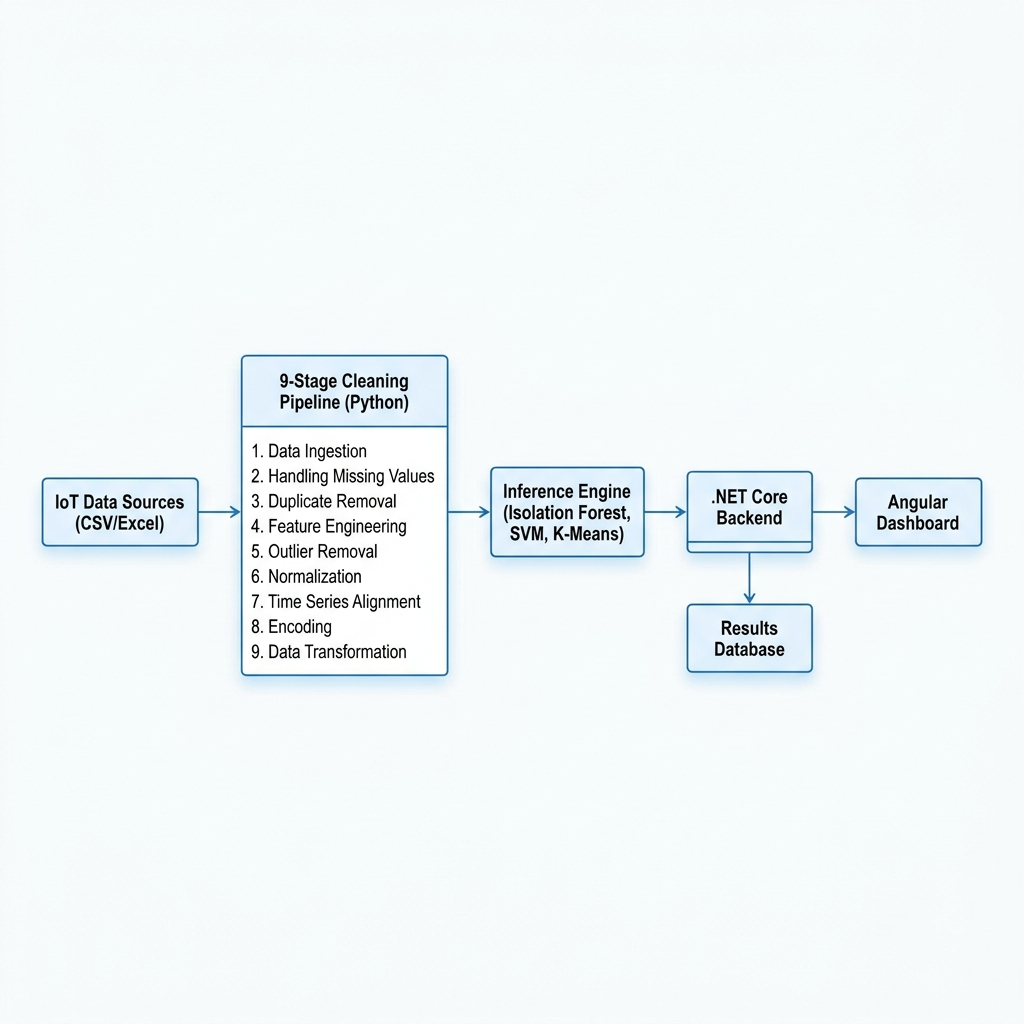
\includegraphics[width=0.9\textwidth]{architecture}
\caption{System Architecture of the IoT Anomaly Detection System.}
\label{fig:architecture}
\end{figure}

\section{Dataset Characteristics and Challenges}
The dataset used in this project represents real-world industrial operations, containing continuous streams of measurements from various machines. The key features collected from the edge devices include:
\begin{itemize}
    \item \textbf{\texttt{RmsStationId} and \texttt{NodeId}}: These values identify exactly which machine or sensor station the data is coming from. 
    \item \textbf{\texttt{LogTypeID} and \texttt{LogSubTypeID}}: These are numerical codes indicating the type of measurement (for example, temperature, humidity, or power consumption). 
    \item \textbf{\texttt{LogFloatValue}}: The actual sensor reading.
    \item \textbf{\texttt{LogTime} and \texttt{ServerTime}}: The exact moment the reading was taken at the machine, and the moment it was received by the central server.
\end{itemize}

One of the biggest challenges with this data is that it is highly imbalanced. In a factory, machines operate normally 99\% of the time, meaning we have millions of "normal" readings but very few examples of "abnormal" readings. Because we do not have enough examples of broken machines to train the system, we cannot use standard supervised learning. Instead, we must use unsupervised learning techniques \cite{kumar2021}, which learn what the normal 99\% looks like and then raise an alarm for anything that behaves differently.


\section{The 9-Stage Data Cleaning Pipeline}
To ensure high data quality, a robust 9-stage cleaning and preprocessing pipeline was implemented in Python. This pipeline ensures that the machine learning models receive consistent and valid data.

\begin{enumerate}
    \item Ensuring required columns (e.g., \texttt{LogTime}, \texttt{LogFloatValue}) exist.
    \item Converting timestamps to datetime objects and sensor values to appropriate numeric types.
    \item Removing or imputing rows with critical missing values.
    \item Eliminating redundant records based on unique sensor/timestamp combinations.
    \item Checking if values fall within realistic physical ranges (e.g., humidity between 0-100\%).
    \item Unlike global outlier detection, this stage computes Interquartile Range (IQR) fences for each specific \texttt{LogType} group. This ensures that a temperature reading is compared only against other temperature readings, preventing false positives caused by differing scales across sensor types.
    \item Feature Engineering:
    \begin{itemize}
        \item Computing the difference between \texttt{ServerTime} and \texttt{LogTime}.
        \item Extracting the hour of the day to capture diurnal patterns.
    \end{itemize}
    \item Scaling features (using StandardScaler) to ensure the models are not biased toward columns with larger numerical ranges.
    \item One-hot encoding categorical variables like \texttt{LogTypeID} to make them usable by the algorithms.
\end{enumerate}

\section{Model Training and Selection}
The system utilizes three unsupervised learning algorithms to provide a comparative view of the data. 

\subsection{Training Strategy}
Since true labels (Anomaly/Normal) are often unavailable, the models are trained in an unsupervised manner on the provided dataset. The models learn the ``normal'' density of the data and assign an anomaly score to each record. 

\subsection{Algorithm Parameters}
The models were configured with specific parameters to handle the factory data accurately:
\begin{itemize}
    \item \textbf{Isolation Forest}: This model isolates anomalies instead of profiling normal data. We set the \texttt{contamination} parameter to 0.05. This simply tells the model that we expect roughly 5\% of the sensor readings to be abnormal \cite{liu2008}.
    \item \textbf{One-Class SVM}: This model tries to draw a boundary around the normal data. We used an RBF (Radial Basis Function) kernel because sensor data patterns are often complex and non-linear. We also set a parameter called `nu` to 0.05, which is an upper limit on the fraction of training errors and a lower limit of the fraction of support vectors, effectively controlling how strict the boundary is \cite{scholkopf2001}.
    \item \textbf{K-Means}: This model groups similar data points together. We set $k=3$ to train the model to look for 3 distinct clusters based on the different types of sensors operating in the factory \cite{jain2010}. If a reading is too far away from any of these clusters, it is flagged as an anomaly.
\end{itemize}

\section{Diagnostic Metric: Network Delay}
A key innovation in this methodology is the inclusion of ``Net Delay'' as a diagnostic metric. By calculating the delay between the device logging time and the server reception time, the system can identify potential network congestion or gateway issues. This data is surfaced alongside the anomaly predictions to give a full picture of system performance.
